\section{Technology Assessment}
\label{sec:technology}

This section explores the key concepts, architecture, and performance characteristics of the chosen authentication technologies: OAuth 2.0 and Basic Authentication. These technologies are evaluated in the context of FeedApp, a system designed to facilitate secure interactions such as creating polls, voting, and managing user-generated content. The primary objective is to assess the scalability and performance of these methods under varying load conditions, ensuring FeedApp's reliability and user experience.

Figure~\ref{fig:framework}, adapted from \cite{brown:96}, provides an overview of the framework used for this evaluation. This structured approach ensures a thorough assessment of both technologies based on their architectural foundations and real-world performance.

\begin{figure}[thb]
	\centering
	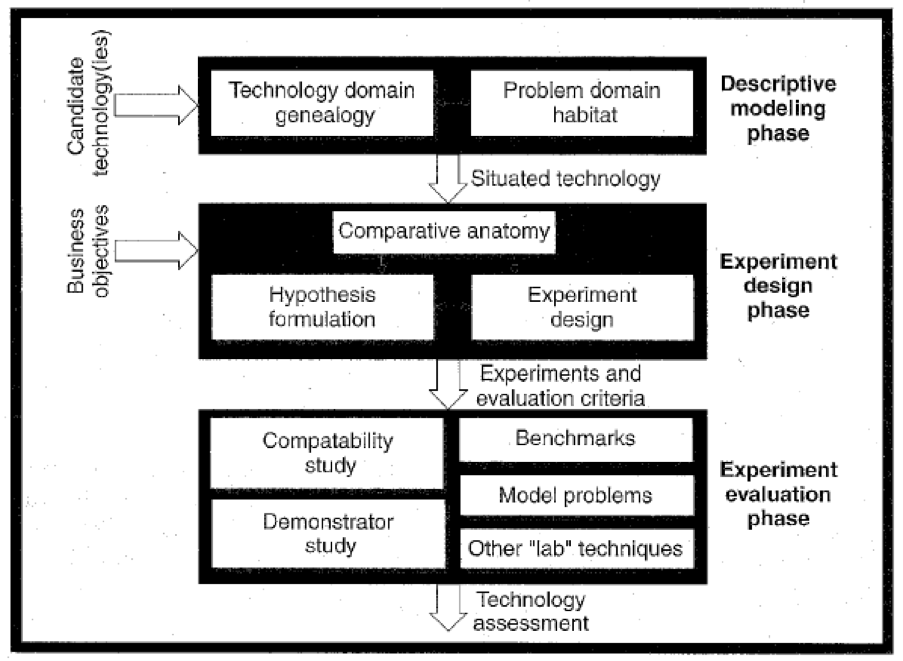
\includegraphics[scale=0.5]{figs/framework.png}
	\caption{Software technology evaluation framework.}
	\label{fig:framework}
\end{figure}

\subsection{Descriptive Modeling}
OAuth 2.0 is a widely used framework for secure user authentication and resource access. It enables systems to delegate access by issuing short-lived access tokens to clients instead of directly sharing user credentials. This token-based approach enhances security by limiting what resources can be accessed and for how long. For instance, in our FeedApp, OAuth 2.0 can be used to ensure that only authenticated users can vote or create surveys, without exposing sensitive data like passwords. It is commonly used by large platforms like Google and Facebook, making it an industry standard for secure APIs.

On the other hand, Basic Authentication is a simpler method where the username and password are included in every request’s header for authentication. Although this method is straightforward to implement, it comes with significant security risks. Credentials are repeatedly transmitted over the network, and there is no inherent mechanism to restrict access or enforce expiration policies. This simplicity makes Basic Authentication suitable for smaller-scale systems or those that are not exposed to public internet traffic.

The purpose of this evaluation is to compare these two technologies in the context of FeedApp and determine whether the additional complexity of OAuth 2.0 is justified for its intended use cases.

\subsection{Experiment Design}
To evaluate the two technologies, we designed experiments that focused on three main hypotheses. First, we hypothesized that Basic Authentication would provide lower average request durations due to its simplicity and better throughput under moderate loads. This expectation was based on its lightweight nature and lack of cryptographic overhead. Second, we anticipated that OAuth 2.0 would outperform Basic Authentication in terms of scalability under higher loads, as it avoids database contention by being stateless. Third, we expected that both methods would experience failures under extreme concurrency but that OAuth 2.0 would fail more gracefully due to its token-based architecture.

The experiments involved simulating various levels of concurrent users, ranging from 50 to 10,000, accessing a protected API endpoint. These requests were designed to replicate real-world interactions, such as retrieving data or performing secure operations. Key metrics, including average request duration, failure rates, and throughput, were recorded to evaluate each method’s performance and scalability.

\subsubsection*{Hypotheses}
The primary goals of this assessment are to compare the performance metrics of Basic Authentication and OAuth 2.0, including average request durations, failure rates, and data overhead. Assess the scalability of each method under increasing load. Provide recommendations for scenarios where each technology would be most effective.

\begin{enumerate}
    \item \textbf{Hypothesis 1}: Performance: Basic Authentication will demonstrate lower average request durations and better throughput under moderate loads due to its simplicity and minimal computational overhead.
    \item \textbf{Hypothesis 2}: Scalability: OAuth 2.0, with its stateless token validation, will outperform Basic Authentication at higher loads by avoiding database contention.
    \item \textbf{Hypothesis 3}: Failure Rates: Both methods will experience failure rates under extreme concurrency, but OAuth 2.0 will fail more gracefully due to its architecture.
\end{enumerate}

\subsection{Experiment Evaluation}

The experimental results provided valuable insights into the strengths and limitations of both authentication methods. At lower loads, both OAuth 2.0 and Basic Authentication performed well, with no significant differences in metrics such as average request durations or failure rates. However, as concurrency increased, clear differences began to emerge.

Basic Authentication demonstrated faster response times and better throughput under moderate loads, owing to its simple design that requires fewer computational steps. However, its reliance on a centralized database for validating credentials became a bottleneck as the number of concurrent users grew. This dependency led to higher latencies and increased failure rates under heavy loads, particularly beyond 1000 virtual users.

In contrast, OAuth 2.0 showed consistent performance up to moderate loads by leveraging its stateless architecture, which avoids frequent database interactions. However, the cryptographic operations required for token validation introduced additional overhead, resulting in higher average request durations. Under extreme concurrency (10,000 virtual users), OAuth 2.0 also experienced significant failures due to resource exhaustion during token validation.

Tables~\ref{tab:performance-comparison} and \ref{tab:scalability-results} summarize the key findings. Table~\ref{tab:performance-comparison} highlights the results for 100 virtual users, showing comparable performance between the two methods. Table~\ref{tab:scalability-results}, however, demonstrates the challenges both methods faced at 3000 virtual users, with Basic Authentication achieving higher throughput but struggling with scalability and OAuth 2.0 encountering significant resource constraints.

\begin{table}[h!]
\centering
\resizebox{\textwidth}{!}{%
\begin{tabular}{|l|c|c|p{6cm}|}
\hline
\textbf{Metric} & \textbf{Basic Authentication (100 VUs)} & \textbf{OAuth 2.0 (100 VUs)} & \textbf{Observations} \\ \hline
\textbf{Data Received (kB/s)}  & 447 kB (15 kB/s)          & 447 kB (15 kB/s)              & Equal amount of data received for both methods.  \\ \hline
\textbf{Data Sent (kB/s)  } & 1.8 MB (61 kB/s)          & 204 kB (6.7 kB/s)             & OAuth sends more data due to token size and overhead.   \\ \hline
\textbf{Average Request Duration (ms)} & 9.96 ms                  & 3.95 ms                       & OAuth takes ~2.5x longer due to token validation overhead.  \\ \hline
\textbf{Minimum Request Duration (µs)} & 504.6 µs                 & 93 µs                         & Basic Auth has a faster minimum response time.            \\ \hline
\textbf{Maximum Request Duration (ms)} & 210.48 ms                & 44.66 ms                      & OAuth has significantly higher maximum response times.  \\ \hline
\textbf{95th Percentile (ms) }  & 22.12 ms                 & 19.84 ms                      & OAuth shows slightly higher tail latency.          \\ \hline
\textbf{Failed Requests } & 0\%                       & 0\%                            & Both methods handled the load without failures.   \\ \hline
\textbf{Requests per Second   }   & 49.31                    & 49.61                         & Throughput is similar for both methods.     \\ \hline
\end{tabular}
}
\caption{Performance Comparison for 100 Virtual Users}
\label{tab:performance-comparison}
\end{table}

\subsubsection*{Scalability Results}

At higher loads, significant differences were observed. Table~\ref{tab:scalability-results} summarizes the scalability test results for Basic Authentication and OAuth 2.0 under extreme loads.



\begin{table}[h!]
\centering
\resizebox{\textwidth}{!}{%
\begin{tabular}{|l|c|c|c|}
\hline
\textbf{Metric}                      & \textbf{Basic Authentication (3000 VUs)} & \textbf{OAuth 2.0 (3000 VUs)} & \textbf{Observations} \\ \hline
\textbf{Average Request Duration}    & 1.19 s                                  & 1.68 s                        & OAuth has higher overhead under load. \\ \hline
\textbf{Failure Rate}                & 5.83\%                                  & 12.11\%                       & OAuth fails more frequently due to resource exhaustion. \\ \hline
\textbf{Requests per Second}         & 1241.61 req/s                           & 940.98 req/s                  & Basic Auth achieves higher throughput. \\ \hline
\textbf{90th Percentile Latency}     & 1.52 s                                  & 2.31 s                        & OAuth has significantly worse tail latency. \\ \hline
\end{tabular}
}
\caption{Scalability Test Results for 3000 Virtual Users}
\label{tab:scalability-results}
\end{table}

\subsubsection*{Observations}
The results of the experiments provided a clear view of how each technology behaves under different conditions. At lower loads, both methods performed well, with minimal differences in average request durations and no failures. Basic Authentication demonstrated slightly faster response times due to its straightforward design, which requires fewer computational steps than OAuth 2.0’s token validation process.

However, as the number of concurrent users increased, differences began to emerge. At 200 to 1000 virtual users, Basic Authentication started to show signs of strain due to its reliance on a centralized database for credential validation. This dependency created bottlenecks as the number of requests grew. In contrast, OAuth 2.0 maintained consistent performance up to 1000 users by leveraging its stateless architecture, which does not require constant interaction with a database.

When the load was increased to extreme levels, such as 3000 and 10,000 concurrent users, both methods experienced significant challenges. Basic Authentication faced severe scalability issues, with failure rates exceeding 75\% at 10,000 users. The database became overwhelmed, leading to high latencies and frequent timeouts. OAuth 2.0, on the other hand, faced bottlenecks in token validation. Although it avoided database contention, the cryptographic operations required for validating tokens proved to be resource-intensive. This resulted in a 100\% failure rate at 10,000 users, indicating that the system was unable to handle such extreme loads without optimization.

Overall, the results show that while Basic Authentication is faster and simpler at low loads, it struggles to scale effectively. OAuth 2.0 offers better scalability at moderate loads but requires additional resources to handle extreme concurrency.

